\documentclass{article}

% Packages for including figures and tables
\usepackage{graphicx}
\usepackage{amsmath}

% Begin the document
\begin{document}

% Title Page
\title{LaTeX Workshop: Figures, Tables, and Citations}
\author{Dalia Kamal Zadeh and Koorosh Komeili Zadeh}
\date{}
\maketitle

\section*{Including Figures and Tables}

\subsection*{Figures}
To include a figure in LaTeX, use the \texttt{figure} environment:
\begin{verbatim}
\begin{figure}
    \includegraphics{image.png}
    \caption{A sample figure}
\end{figure}
\end{verbatim}

Example usage in the document:
\begin{figure}[h]
    \centering
    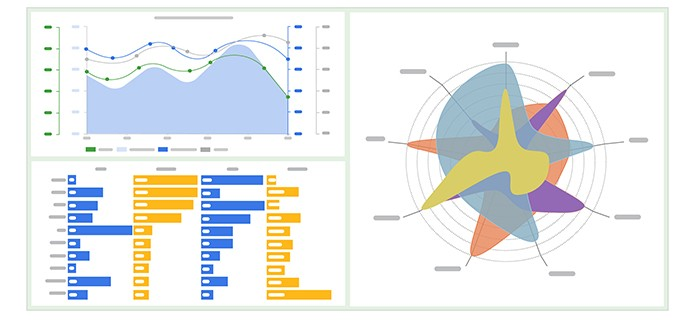
\includegraphics[width=0.9\textwidth]{Figures/sample-chart} % Replace with your file
    \caption{A sample figure}
\end{figure}

\newpage

\subsection*{Tables}
Tables in LaTeX are created using the \texttt{tabular} environment. You can create tables with various types of data, including text, numbers, and percentages, and even format them for readability.

\begin{verbatim}
\begin{tabular}{|c|c|c|c|}
    \hline
    Name & Age & Score & Improvement (\%) \\
    \hline
    Alice & 21 & 85 & 5.5 \\
    Bob & 22 & 90 & 7.2 \\
    Charlie & 20 & 78 & 4.1 \\
    Diana & 23 & 92 & 6.8 \\
    \hline
\end{tabular}
\end{verbatim}

Here is how it looks:

\begin{table}[h]
    \centering
    \begin{tabular}{|c|c|c|c|}
        \hline
        \textbf{Name} & \textbf{Age} & \textbf{Score} & \textbf{Improvement (\%)} \\
        \hline
        Alice & 21 & 85 & 5.5 \\
        Bob & 22 & 90 & 7.2 \\
        Charlie & 20 & 78 & 4.1 \\
        Diana & 23 & 92 & 6.8 \\
        \hline
    \end{tabular}
    \caption{Sample table with fictional data}
\end{table}

Tables can be customized further with more formatting options, colors, and styles.

\newpage

\section*{Bibliography and Citations}

In LaTeX, managing references and citations is streamlined using \texttt{BibTeX}, allowing automatic formatting and management of your bibliography.

\subsection*{Using BibTeX}
To include a bibliography in your document, add the following commands where you want the bibliography to appear:
\begin{verbatim}
\bibliography{references}
\bibliographystyle{plain}
\end{verbatim}
This will pull references from a separate \texttt{references.bib} file, which should be stored in the same directory or properly referenced.

\subsection*{Citations}
Citations are made easily by placing the reference key inside the command like this:
\begin{verbatim}
\cite{reference}
\end{verbatim}

\subsection*{Sample Citations}
Here are some examples of how you can cite notable works:

\begin{quote}
    \centering
    “Raise your quality standards as high as you can live with, avoid wasting your time on routine problems, and always try to work as closely as possible at the boundary of your abilities. Do this, because it is the only way of discovering how that boundary should be moved forward.” \cite{dijkstra1982selected}
\end{quote}

\begin{quote}
    \centering
    "The dominant sequence transduction models are based on complex recurrent or convolutional neural networks that include an encoder and a decoder. The best performing models also connect the encoder and decoder through an attention mechanism. We propose a new simple network architecture, the Transformer, based solely on attention mechanisms, dispensing with recurrence and convolutions entirely." \cite{vaswani2017attention}
\end{quote}


% Bibliography section (BibTeX file would be used here)
\bibliographystyle{plain}
\bibliography{references}  % references.bib file should be created with entries

\end{document}
